\documentclass[12pt]{beamer}
\usepackage{pgf,pgfarrows,pgfnodes,pgfautomata,pgfheaps}
\usepackage{amsmath,amssymb}
\usepackage{graphics}
\usepackage{multimedia}
\usepackage{multimedia}
\usepackage{mcode}

\usepackage{xeCJK}
%\usepackage{fontspec}
\setCJKmainfont[BoldFont=simhei.ttf]{simsun.ttf}
\setCJKsansfont{simhei.ttf}
\setCJKmonofont{simfang.ttf}

%\setCJKmainfont{Adobe Song Std}
%\setCJKmainfont[BoldFont=Adobe Heiti Std]{Adobe Song Std}
%%%%%%%%%%%%%%%%%%%%%%%%%%%%%%%%%%%%%%%%%%%%%%%%%%%%%%
\graphicspath{{figures/}}


\begin{document}
\title{无网格计算方法的网格搜索方法}
\author{周吕文}
\date{2010年11月5日}
\maketitle

\section{Linked-list cells方法}

\frame[<+->]{\frametitle{Linked-list cells方法}

\begin{columns}
\begin{column}[c]{0.35\textwidth}
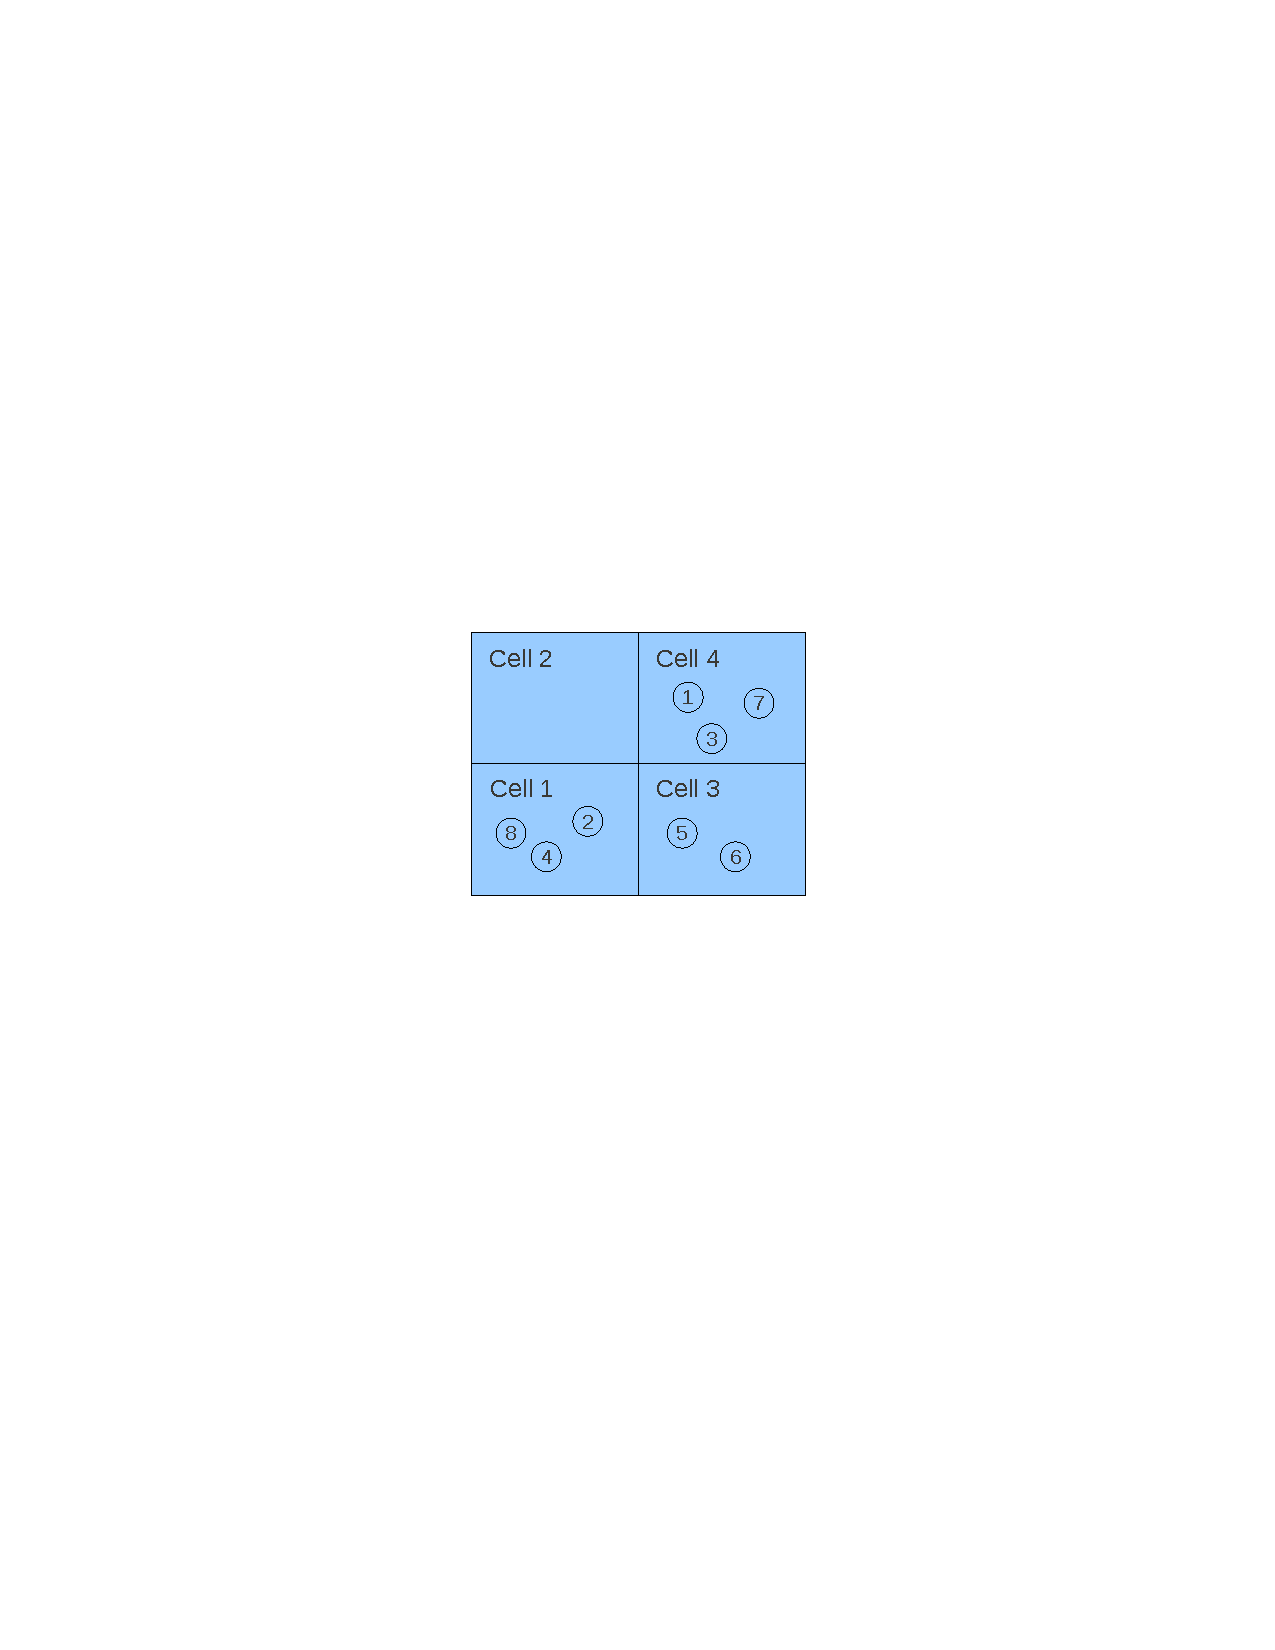
\includegraphics[width=\textwidth]{fig01.pdf}
\end{column}
\begin{column}[c]{0.65\textwidth}
\begin{center}
{\small
\begin{tabular}{lllllllll}
 & 1 & 2 & 3 & 4 &  &  &  &  \\
\cline{2-5}
\multicolumn{1}{l|}{Head} & \multicolumn{1}{l|}{8} & \multicolumn{1}{l|}{0} & \multicolumn{1}{l|}{6} & \multicolumn{1}{l|}{7} &  &  &  &  \\
\cline{2-5}
 & 1 & 2 & 3 & 4 & 5 & 6 & 7 & 8 \\
\cline{2-9}
\multicolumn{1}{l|}{Link} & \multicolumn{1}{l|}{0} & \multicolumn{1}{l|}{0} & \multicolumn{1}{l|}{1} & \multicolumn{1}{l|}{2} & \multicolumn{1}{l|}{0} & \multicolumn{1}{l|}{5} & \multicolumn{1}{l|}{3} & \multicolumn{1}{l|}{4} \\
\cline{2-9}
\end{tabular}
}
\end{center}
\end{column}
\end{columns}

\textcolor{white}{.}

\pause 通过Head和Link来访问某个格子中所有的粒子,如访问第4个格子中的粒子:
\begin{itemize}
\item Head(4) = 7 找到第4个格子中最大号粒子即7号粒子
\item Link (7) = 3 找到第4个格子中次大号粒子即3号粒子
\item Link (3) = 1 找到第4个格子中次大号粒子即1号粒子
\item Link (1) = 0 0表示第4个格子中没有其它可搜索粒子
\end{itemize}

}




\frame{\frametitle{生成Link和Head数组的伪代码}

\begin{center}
\begin{tabular}{|lll|}
\hline
\multicolumn{3}{|l|}{Algorithm 1:  Generate Head and Link arrays} \\
\hline
\multicolumn{3}{|l|}{Initialize Link and Head} \\
\multicolumn{3}{|l|}{Do for all particles i form 1 to n} \\
 &       & Icell = The number of cell which contain  particle i \\
  &       & \\
 &  & \textcolor{blue}{! Link to the previous occupant } \\
 &  &  Link(i) = Head(Icell) \\
   &       & \\
 &  & \textcolor{blue}{! The last one goes to the header } \\
 &  & Head(Icell) = i \\
\multicolumn{3}{|l|}{End do} \\
\hline
\end{tabular}
\end{center}
}


\frame{\frametitle{访问某一格子中粒子的伪代码}
\begin{center}
\begin{tabular}{lll}
\hline
\multicolumn{3}{|l|}{Algorithm 2:  Access All Particle in One Cell} \\
\hline
\multicolumn{3}{|l|}{i = Head(Number of one cell)} \\
\multicolumn{3}{|l|}{Do while I not equal 0} \\
\multicolumn{1}{|l}{} &  & \multicolumn{1}{l|}{Access the i-th particle} \\
\multicolumn{1}{|l}{} &  & \multicolumn{1}{l|}{i = Link(i)} \\
\multicolumn{3}{|l|}{End do} \\
\hline
\end{tabular}
\end{center}
}

\section{Data locality 方法}
\frame{\frametitle{Data locality 方法}
\begin{columns}
\begin{column}[c]{0.35\textwidth}
\begin{center}
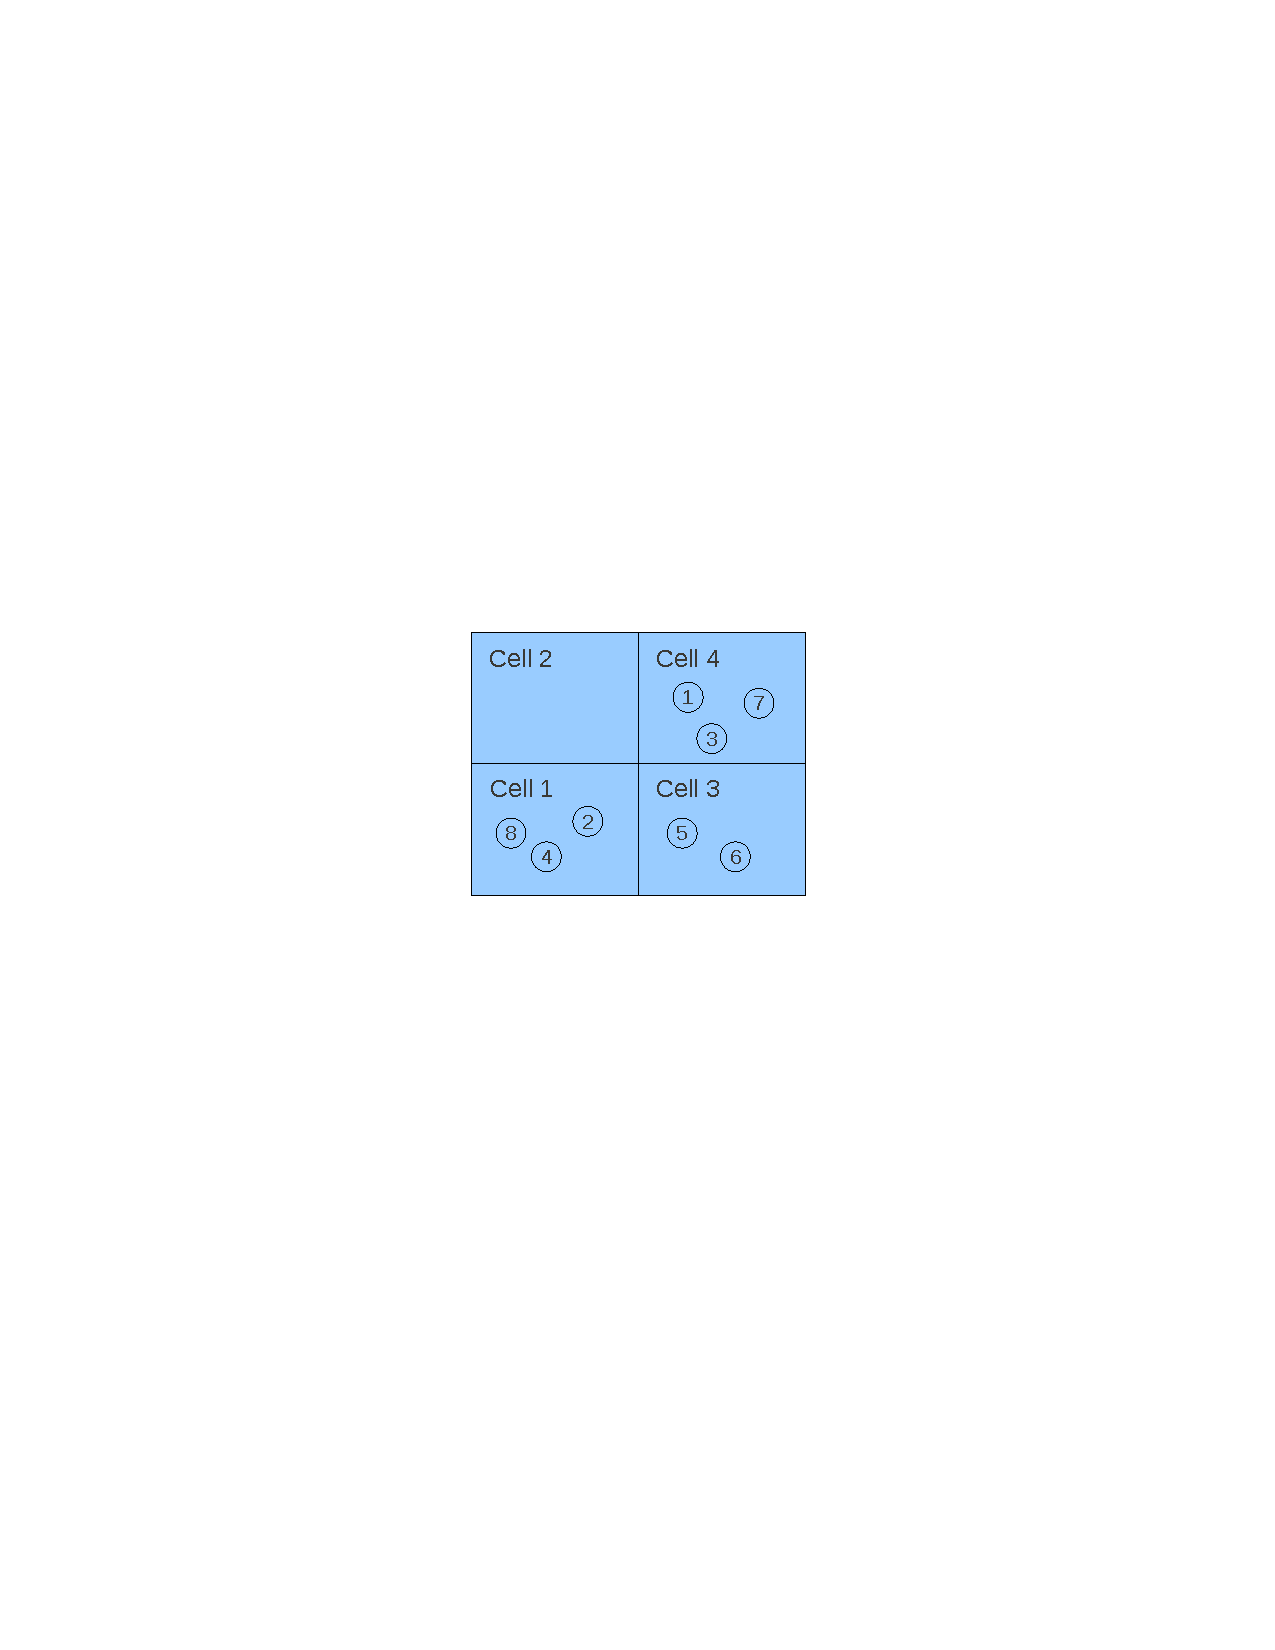
\includegraphics[width=\textwidth]{fig01.pdf}
\end{center}
\end{column}
\begin{column}[c]{0.65\textwidth}

{\footnotesize
\begin{tabular}{lllllllll}
 & 1 & 2 & 3 & 4 & 5 & 6 & 7 & 8 \\
\cline{2-9}
\multicolumn{1}{l|}{OldList} & \multicolumn{1}{l|}{1} & \multicolumn{1}{l|}{2} & \multicolumn{1}{l|}{3} & \multicolumn{1}{l|}{4} & \multicolumn{1}{l|}{5} & \multicolumn{1}{l|}{6} & \multicolumn{1}{l|}{7} & \multicolumn{1}{l|}{8} \\
\cline{2-9}
 & 1 & 2 & 3 & 4 & 5 & 6 & 7 & 8 \\
\cline{2-9}
\multicolumn{1}{l|}{NewList} & \multicolumn{1}{l|}{\textcolor{red}{2}} & \multicolumn{1}{l|}{\textcolor{red}{4}} & \multicolumn{1}{l|}{\textcolor{red}{8}} & \multicolumn{1}{l|}{5} & \multicolumn{1}{l|}{6} & \multicolumn{1}{l|}{\textcolor{blue}{1}} & \multicolumn{1}{l|}{\textcolor{blue}{3}} & \multicolumn{1}{l|}{\textcolor{blue}{7}} \\
\cline{2-9}
 & 1 & 2 & 3 & 4 & 5 &  &  &  \\
\cline{2-6}
\multicolumn{1}{l|}{CellEnd} & \multicolumn{1}{l|}{0} & \multicolumn{1}{l|}{3} & \multicolumn{1}{l|}{3} & \multicolumn{1}{l|}{5} & \multicolumn{1}{l|}{8} &  &  &  \\
\cline{2-6}
\end{tabular}}
\end{column}
\end{columns}

\textcolor{white}{.}\\
\textcolor{white}{.}

用CellEnd数组存放每个格子中所用粒子在NewList中的位置, 第i个格子中的所用粒子表示为
\[
CellEnd(i)+1 \cdots CellEnd(i+1)
\]
}

\frame{\frametitle{生成NewList和CellEnd数组的伪代码}

\begin{center}
\begin{tabular}{lll}
\hline
\multicolumn{3}{|c|}{Algorithm 3:  Generate NewList and CellEnd arrays} \\
\hline
\multicolumn{3}{|l|}{Initialize NewList,  CellEnd and Temp} \\
\multicolumn{3}{|c|}{} \\
\multicolumn{3}{|l|}{\textcolor{blue}{! Generate CellEnd array}} \\
\multicolumn{3}{|l|}{Do for all particles i form 1 to n} \\
\multicolumn{1}{|l}{} &  & \multicolumn{1}{l|}{Icell = The index of cell which contain  particle i} \\
\multicolumn{1}{|l}{} &  & \multicolumn{1}{l|}{CellEnd(Icell+1:end) = CellEnd(Icell+1:end) +1} \\
\multicolumn{3}{|l|}{End do} \\
\multicolumn{3}{|l|}{} \\
\multicolumn{3}{|l|}{\textcolor{blue}{! Generate NewList array}} \\
\multicolumn{3}{|l|}{Temp = CellEnd} \\
\multicolumn{3}{|l|}{Do for all particles i from n to 1} \\
\multicolumn{1}{|l}{} &  & \multicolumn{1}{l|}{Icell = The index of cell which contain  particle i} \\
\multicolumn{1}{|l}{} &  & \multicolumn{1}{l|}{ NewList( Temp(Icell+1) ) = I} \\
\multicolumn{1}{|l}{} &  & \multicolumn{1}{l|}{Temp(Icell+1) = Temp(Icell+1)  - 1} \\
\multicolumn{3}{|l|}{End do} \\
\hline
\end{tabular}
\end{center}
}


\frame{\frametitle{访问某一格子中粒子的伪代码}

\begin{center}
\begin{tabular}{lll}
\hline
\multicolumn{3}{|l|}{Algorithm 4:  Access All Particle in One Cell} \\
\hline
\multicolumn{3}{|l|}{Do for i form CellEnd(c)+1 to CellEnd(c+1)} \\
\multicolumn{1}{|l}{} &  & \multicolumn{1}{l|}{access particle NewList(i)} \\
\multicolumn{3}{|l|}{End do} \\
\hline
\end{tabular}
\end{center}
}


\section{半邻居网格搜索}

\frame{\frametitle{格子的编号}

\begin{columns}
\begin{column}[c]{0.5\textwidth}
\begin{center}
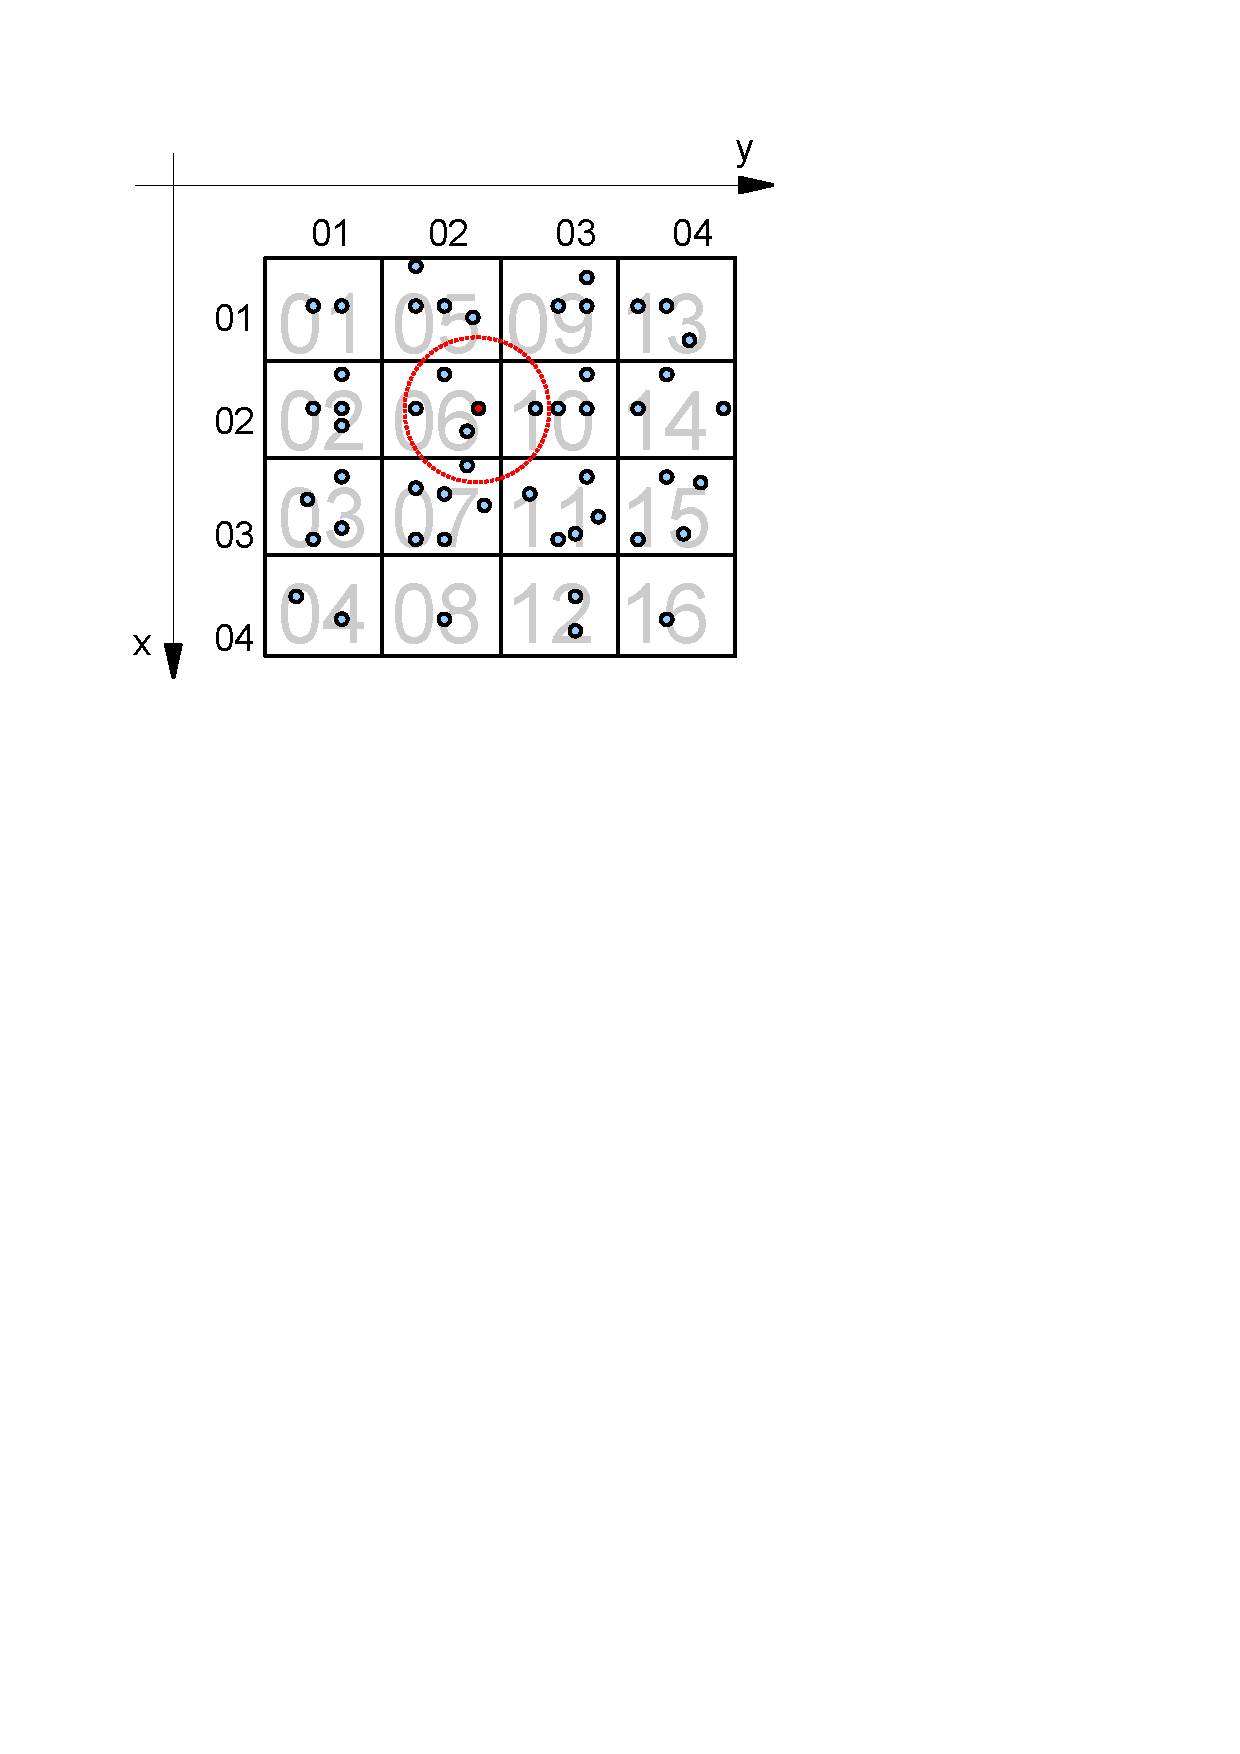
\includegraphics[width=\textwidth]{fig02.pdf}
\end{center}
\end{column}
\begin{column}[c]{0.5\textwidth}

\[
r =\left[
\begin{array}{c}
  r_1 \\
  r_2 \\
  \vdots \\
  r_n
\end{array}\right]=
\left[
\begin{array}{cc}
  x_1 & y_1 \\
  x_2 & y_2 \\
  \vdots & \vdots \\
  x_n & y_n
\end{array}\right]
\]

\[
boxl = [L_x, L_y], Nc =[Nc_x, Nc_y]
\]
\end{column}
\end{columns}

\textcolor{white}{.}

\[
CellSub_i = \Big[\lfloor  \frac{x_i}{Nc_x}\cdot L_x\rfloor, \lfloor  \frac{y_i}{Nc_y}\cdot L_y\rfloor \Big] + 1
\]

\[
CellInd_i = \Big[CellSub_i - [0, 1]\Big]\left[
                                \begin{array}{c}
                                  1  \\
                                  Nc_x  \\
                                \end{array}
                              \right]
\]
}


\frame{\frametitle{搜索网格}
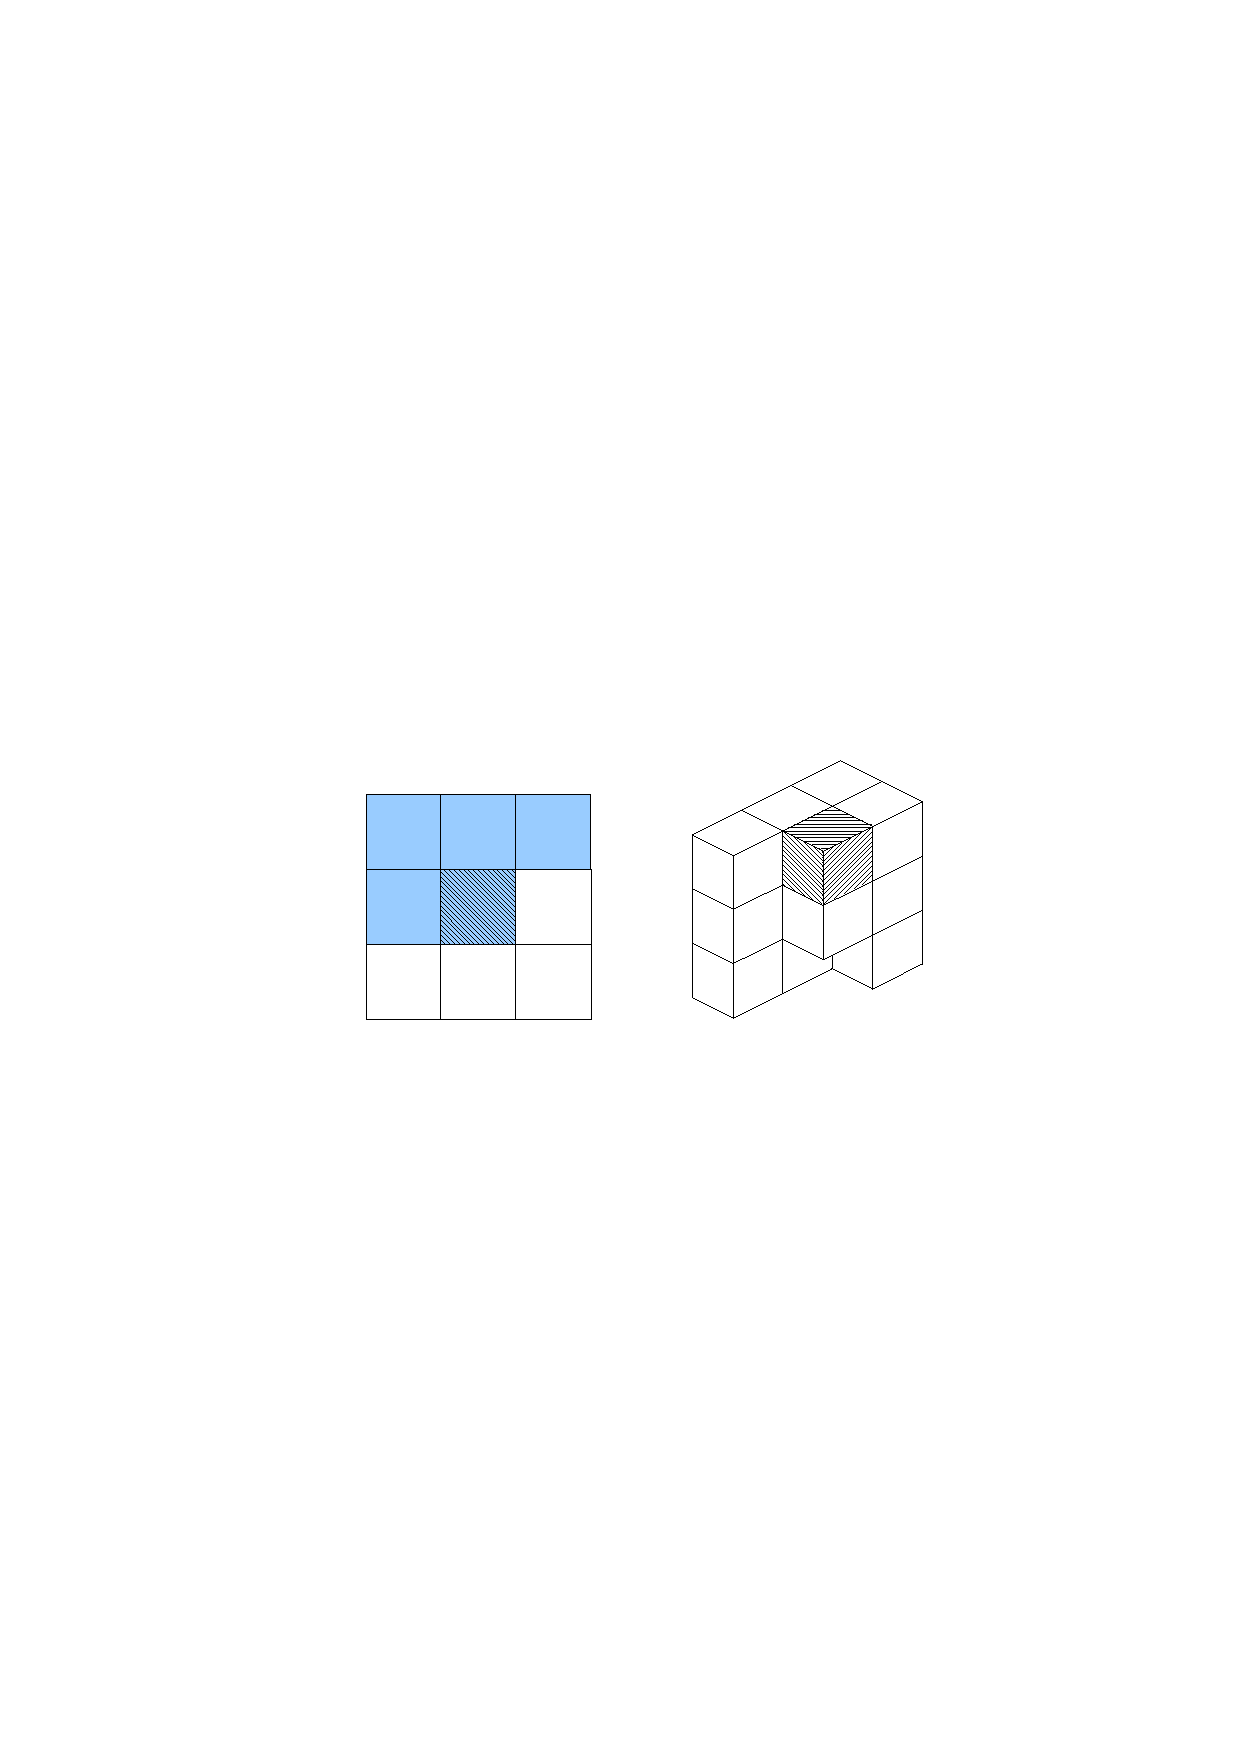
\includegraphics[width=\textwidth]{fig03.pdf}


}


\frame{\frametitle{搜索网格}

{\scriptsize
\begin{tabular}{|l|ll|ll|lllll}
\hline
\multicolumn{10}{|l|}{Algorithm 5: half neighbors search base on Linked-list Cells (3D)} \\
\hline
\multicolumn{10}{|l|}{\textbf{Do} for all cells i} \\
 &  & \multicolumn{8}{l|}{CellInd\_i = i} \\
 &  & \multicolumn{8}{l|}{atom\_i = Head(CellInd\_i)} \\
 &  & \multicolumn{8}{l|}{\textcolor{blue}{Do} while atom\_i not equal 0} \\
 &  &  &  & \multicolumn{6}{l|}{\textcolor{red}{Do} for all 14 cells j in the neighborhood of cell i} \\
 &  &  &  &  &  & \multicolumn{4}{l|}{ CellInd\_j = Index of cells j} \\
 &  &  &  &  &  & \multicolumn{4}{l|}{If  CellInd\_i equal CellInd\_j  then} \\
 &  &  &  &  &  &  &  & \multicolumn{2}{l|}{atom\_j = Link(atom\_i)} \\
 &  &  &  &  &  & \multicolumn{4}{l|}{Else} \\
 &  &  &  &  &  &  &  & \multicolumn{2}{l|}{atom\_j = head(CellInd\_j)} \\
 &  &  &  &  &  & \multicolumn{4}{l|}{End if} \\
 &  &  &  &  &  & \multicolumn{4}{l|}{Do while atom\_j not equal 0} \\
 &  &  &  &  &  &  &  & \multicolumn{2}{l|}{\textcolor{blue}{!*******************************************}} \\
 &  &  &  &  &  &  &  & \multicolumn{2}{l|}{compute the force between atom\_i and atom\_j in here} \\
 &  &  &  &  &  &  &  & \multicolumn{2}{l|}{\textcolor{blue}{!*******************************************}} \\
 &  &  &  &  &  &  &  & \multicolumn{2}{l|}{ atom\_j = link(atom\_j)} \\
 &  &  &  &  &  & \multicolumn{4}{l|}{End do} \\
 &  &  &  & \multicolumn{6}{l|}{\textcolor{red}{End do}} \\
 &  &  &  & \multicolumn{6}{l|}{atom\_i = Link(atom\_i)} \\
 &  & \multicolumn{8}{l|}{\textcolor{blue}{End do }} \\
\multicolumn{10}{|l|}{\textbf{End do}} \\
\hline
\end{tabular}
}
}


\frame{
\begin{center}
{\Huge
THE END
}
\end{center}

}
\end{document}
